\documentclass[10pt,a4paper]{article}
\usepackage[utf8]{inputenc}
\usepackage[T1]{fontenc}
\usepackage{graphicx}
\usepackage[usenames, dvipsnames]{xcolor}
\usepackage{float}
\usepackage{mathtools}
\usepackage{amsmath}
\usepackage{amsfonts}
\usepackage{amsthm}
\usepackage{thmtools}
\usepackage{enumitem}
\theoremstyle{definition}
\newtheorem{definition}{Definition}[part]
\newtheorem{subdefinition}{Definition}[definition]

\declaretheorem[sibling=definition, shaded={rulecolor=black, rulewidth=0.8pt, 
	bgcolor={rgb}{1,1,1}},name=Definition]{boxeddef}
\declaretheorem[sibling=subdefinition, shaded={rulecolor=black, rulewidth=0.5pt, 
	bgcolor={rgb}{1,1,1}},name=Definition]{boxedsubdef}

\theoremstyle{plain}
\newtheorem{example}{Example}[definition]


\title{Machine Learning 2023}
\author{David Graf}
\date{\today}
\begin{document}
	\maketitle
\part{Actual ML lecture content}
Recap of our setup:
\begin{enumerate}
	\item DOMAIN set X; we call $x\in X$ an instance
	\item LABEL set Y; e.g. $Y = \{0, 1\}$ (for a binary problem)
	\item TRAINING set $\mathcal{S} = \big((x_1, y_1), ..., (x_m, y_m)\big)$  with $x_i \in X, y_i \in Y$
	\item a LEARNER that receives $\mathcal{S}$ and outputs 
	$$ h: X \to Y$$
	which we call a hypothesis
\end{enumerate}
Assumption: for now, we assume $x_i$'s are drawn iid from some probability measure $\mathcal{D}$ over the domain and labelled by some function (the labelling function) $f: X \to Y$:
$$ x_i \underbrace{ \sim }_{\text{\scriptsize"drawn from"}} \mathcal{D},\ y_i = f(x_i)$$

We are "interested" in 
$$\mathcal{D}(\{x \in X: h(x) \neq f(x) \}) = \mathbb{P}_{X \sim \mathcal{D}}[h(x) \neq f(x)] = L_{\mathcal{D}, f}(h)$$
$L_{\mathcal{D}, f}(h)$ is called the "Generalization Error" or "Risk".\\
\newline
The \underline{empirical version} of this is 
\begin{equation}
	\tag{[m] = \{1, ..., m\}}
	\frac{1}{m}\cdot\big|\big\{ i \in [m]: h(x_i) \neq f(x_i) \big\}\big| = L_\mathcal{S}(h)
\end{equation}
the empirical error or empirical risk $L_\mathcal{S}(h)$.
\paragraph{Convention:}
$\mathcal{S}|_x = (x_1,..., x_m)$

\paragraph{Claim:}
ADD COMMENTS ON THE SIDE HERE, SLIDE 27
\begin{align*}
 \mathbb{E}_{\mathcal{S}|_x \sim \mathcal{D}^m}[L_\mathcal{S}(H)] &= \mathbb{E}_{\mathcal{S}|_x}\bigg[\frac{1}{m} \cdot \sum_{i=1}^{m} 1_{h(x_i) \neq f(x_i)}\bigg]\\
 &= \frac{1}{m} \cdot \sum_{i=1}^{m} \mathbb{E}_{x_i \sim \mathcal{D}}[1_{h(x_i) \neq f(x_i)}] && \text{(by linearity of $\mathbb{E}$)}\\
 &= \frac{1}{m} \cdot \sum_{i=1}^{m} \mathbb{E}_{X \sim \mathcal{D}}[1_{h(x) \neq f(x)}]\\
 &= \frac{1}{m} \cdot \sum_{i=1}^{m} \mathbb{P}_{X\sim \mathcal{D}}[1_{h(x) \neq f(x)}]\\
 &=  \frac{1}{m} \cdot m \cdot \mathbb{P}_{X\sim \mathcal{D}}[1_{h(x) \neq f(x)}]\\
 &= L_{\mathcal{D},f}(h)
\end{align*}

\paragraph{Our first learning paradigm} \underline{Empirical risk minimization (ERM)}:\\
As we only have access to the training data (S), it's natural to try to select \underline{h} such that the empirical risk is minimized. We call such an h an \underline{empirical risk minimizer} $(h_S)$.\\

\underline{A problematic case:}
\begin{figure}[H]
	\centering
	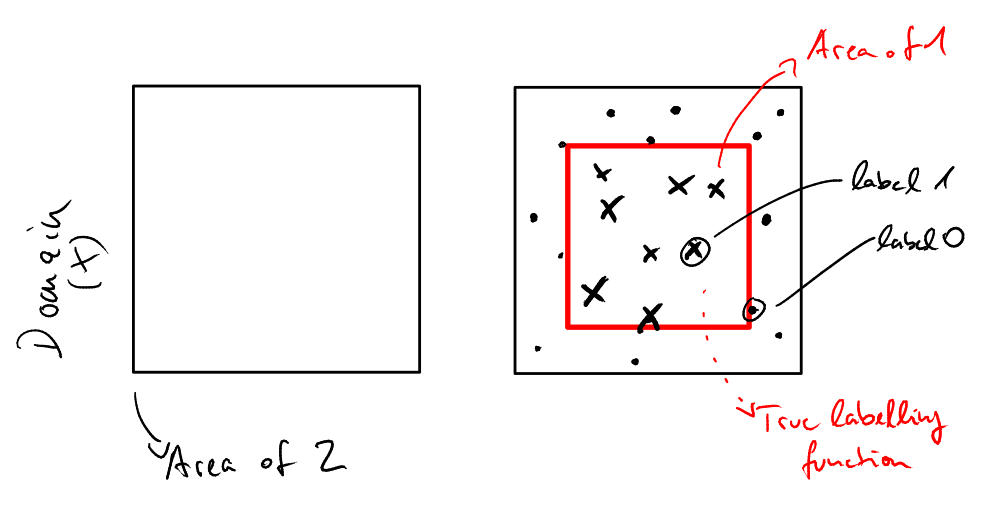
\includegraphics[width=0.7\linewidth]{sketch_1}
	\caption{Problematic Case 1}
	\label{fig:sketch1}
\end{figure}

\begin{itemize}
	\item say the distribution on X is uniform
	\item say we have an ERM algorithm that returns $h_S$ such that 
	\begin{align*}
			 h_s(x) &= \begin{cases}
			y_i , &  \text{if } \exists \ i \in [m]: x_i = x  \\
			0 , &  \text{else} 
		\end{cases} && \text{(a lookup table)} 
	\end{align*}
	Obviously $h_S$ is correct on our training set $$\implies L_S(h_S) = 0\text{ !}$$
	But on unseen instances from $D (X \sim D)$, $h_S$ is only correct 50\% of the time (due to the ratio of the areas of the black and red squares in the sketch): $$\implies L_{D,f}(h_S) = \frac{1}{2} \text{ !}$$
	This is called overfitting.
\end{itemize}

\paragraph{Hypothesis class (H):} We restrict searching for h to H, i.e., a class of functions from X to Y, and write:
$$
\text{ERM} = \text{ERM}_{H} (\mathcal{S}) \in \text{argmin}_{h \in H} L_{\mathcal{S}}(h)
$$
\underline{Remark:} In our previous example, we did not do this and allowed to memorize the training data!

\paragraph{ERM over finite hypothesis classes $(\big|H\big| < \infty)$:} 
$$\text{\underline{Assumption (realizability):} } \exists \ h^*\in H \text{ with } L_{\mathcal{D},f}(h^*) = 0$$
Now, any ERM hypothesis $h_\mathcal{S}$ will attain 0 empirical error ($L_\mathcal{S}(h_\mathcal{S}) = 0$), as it computes with $h^*$ (which obviously has 0 empirical error).\\
\newline
Hence, $L_{\mathcal{D},f}(h_\mathcal{S}) > \varepsilon$ can only happen if we select a hypothesis with $L_\mathcal{S}(h_\mathcal{S}) = 0$ but $L_{\mathcal{D},f}(h_\mathcal{S}) > \varepsilon$ (trivially). We can write
\begin{align*}
	H_\text{\textbf{bad}} = \{h \in H: L_{D,f}(h)>\varepsilon\} && \text{ set of \textbf{bad} hypotheses}
\end{align*}
Also, we define
$$
	M = \{\mathcal{S}|_x : \exists h \in \underbrace{H_{\mathrm{\textbf{bad}}}}_{\mathclap{\text{those are the ones with generalization error $> \varepsilon$}}}, L_\mathcal{S}(h) = 0  \}
$$

We observe
$$
\big\{\mathcal{S}|_x : L_{\mathcal{D},f}(\underbrace{h_\mathcal{S}}_{\mathclap{\text{ERM}}}) \geq \varepsilon\big\} \subseteq  \underbrace{\big\{\mathcal{S}|_x : \exists \ h \in H_{\mathrm{\textbf{bad}}}, L_\mathcal{S}(h) = 0 \big\}}_{\mathclap{M = \cup_{h \in H_{\mathrm{\textbf{bad}}}}\{\mathcal{S}|_x: L_{\mathcal{S}}(h) = 0\} }} = M
$$

We get (upon measuring with $\mathcal{D}$):
\begin{align*}
\mathcal{D}^m \big( \{\mathcal{S}|_x : L_{\mathcal{D},f}(h_\mathcal{S}) \geq \varepsilon\}\big) &\leq \mathcal{D}^m\big( \cup_{h \in H_{\mathrm{\textbf{bad}}}}\{\mathcal{S}|_x : L_{\mathcal{S}}(h) = 0\} \big)\\
&\leq \sum_{h \in H_{\mathrm{\textbf{bad}}}} \mathcal{D}^m \big(\{\mathcal{S}|_x : L_{\mathcal{S}}(h) = 0\}\big) && \text{(due to $\sigma$-sub-additivity)}
\end{align*}
\underline{Let's fix some $h \in H_{\mathrm{\textbf{bad}}}$:}
\begin{align*}
	D^m \big(\{\mathcal{S}|_x : L_{\mathcal{S}}(h) = 0\}\big) &= \mathcal{D}^m \big(\{\mathcal{S}|_x : \forall i \in [m]: h(x_i) = f(x_i)\}\big)\\
	&= \prod_{i = 1}^{n} \mathcal{D} \big(\{x_i: h(x_i) = f(x_i)\}\big) && \text{(due to iid assumption)}\\
	&= \prod_{i=1}^{n} (1 - L_{\mathcal{D},f}(h))\\
	&\leq \prod_{i=1}^{n} (1-\varepsilon) && \text{(as $h \in H_{\mathrm{\textbf{bad}}}$)}\\
	&= (1-\varepsilon)^m \\
	&\leq e^{-\varepsilon m}
\end{align*}
So, to conclude:
\begin{align*}
	D^m \big(\{\mathcal{S}|_x : L_{\mathcal{D},f}(h_S) \geq \varepsilon\}\big) &\leq \sum_{h \in H_{\mathrm{\textbf{bad}}}} e^{-\varepsilon m} \\ 
	&= |H_{\mathrm{\textbf{bad}}}| \cdot e^{-\varepsilon m} \\
	&\leq |H| \cdot e^{-\varepsilon m}
\end{align*}
This is a probabilistic guarantee that tells us how the generalization error scales with the sample size. If we increase m, ew can make $\varepsilon$ arbitrarily small. 
If we let $ |H| \cdot e^{-\varepsilon m} <\delta \in (0,1)$ and solve for $m$, we get 
$$ m>\frac{1}{\underbrace{\colorbox{orange}{$\varepsilon$}}_{error}} \cdot \log \Big(\frac{|H|}{\underbrace{\colorbox{orange}{$\delta$}}_{confidence}}\Big)$$
\paragraph{Corollary:} Let $|H| < \infty$ and $\varepsilon, \delta \in (0,1)$. Let $m$ be an integer (the sample size) such that $\color{red} m>\frac{1}{\varepsilon} \cdot log \big(\frac{|H|}{\delta}\big)$. Then, for each labeling function $f: X \to Y$ and any distribution $\mathcal{D}$ over domain $X$ (for which realizability holds), we have that with probability of at least $1-f$ over the choice of $S|_x$ (of size m) it holds that every ERM hypothesis $h_s$ satisfies the following:
$$ L_{\mathcal{D},f} \leq \varepsilon $$

\textcolor{red}{\paragraph{Interpretation:} For sufficiently large $m, ERM_H$ returns $h_S$ (i.e., a hypothesis) that is \textbf{P}ROBABLY \textbf{A}PPROXIMATELY \textbf{C}ORRECT (PAC).}\\
\newline
This leads to:
\begin{boxeddef}[PAC learnability]
	A hypothesis class $H$ is \textcolor{red}{PAC learnable}, if there exists a function $m_H: (0,1)^2 \to \mathbb{N}$ and a learning algorithm $\mathcal{A}$ with the following properties:
	\begin{enumerate}
		\item for every $\varepsilon, \delta \in (0,1)$ and
		\item every distribution $\mathcal{D}$ over domain $\mathcal{X}$ and
		\item every labelling function $f: X \to \{0, 1\}$ if
		\item realizability holds (w.r.t. to $\mathcal{D}, H, f$) then
	\end{enumerate}
	running $\mathcal{A}$ on $m \geq m_H(\varepsilon, \delta)$ \textit{iid.} instances drawn from $\mathcal{D}$ and labelled by $f$, returns a hypothesis $h$ such that with probability of at least $1-\delta$ (over choice of S) 
	$$ L_{\mathcal{D}, f} \leq \varepsilon $$
\end{boxeddef}
\begin{boxedsubdef}[Sample complexity]
	$m_H: \{0,1\} \to \mathbb{N}$ is called the \textcolor{red}{sample complexity} function. In particular, $m_H$ returns the smallest integer such that the requirements for PAC-learnability are satisfied
\end{boxedsubdef}
We have already seen that \textcolor{red}{finite hypothesis classes} ($|H| < \infty$) \textcolor{red}{are PAC learnable} with 
$$ m_H(\varepsilon, \delta) \leq \bigg\lceil\frac{1}{\varepsilon} \cdot log \bigg( \frac{|H|}{\delta}\bigg) \bigg\rceil $$

We will now move to a more general setting.
\begin{enumerate}[label*=\protect\fbox{\arabic{enumi}}]
	\item We will first release the realizability assumption (In this setting, the best we can hope for are guarantees relative to the "best" possible hypothesis in the class: $$\min_{h \in H}{L_{\mathcal{D}, f}(h)}$$
\end{enumerate}
	\begin{boxeddef}[Höffding inequality]
	Let $X_1, ..., X_m$ be \textit{iid} random variables taking values in $[a_i, b_i]$ for $i \in [m]$. Then, it holds that
	 \begin{align*}
	 	\mathbb{P}\bigg[S_m - \mathbb{E}[S_m] > \varepsilon\bigg] &\leq e^{\frac{-2 \varepsilon^2}{\sum_{i} (b_i - a_i)^2}} && , S_m = \sum_{i = 1}^{m} X_i, &&& \text{and}\\
	 	\mathbb{P}\bigg[S_m - \mathbb{E}[S_m] < -\varepsilon\bigg] &\leq e^{\frac{-2 \varepsilon^2}{\sum_{i} (b_i - a_i)^2}} 
	\end{align*}
	Also:
	\begin{align*}
	 	\mathbb{P}\bigg[\big|S_m - \mathbb{E}[S_m]\big| > \varepsilon\bigg] &\leq 2 \cdot e^{\frac{-2 \varepsilon^2}{\sum_{i} (b_i - a_i)^2}}\\
	 	HIER NOTIZ EINFÜGEN
	 \end{align*}

\end{boxeddef}
Another useful form of this inequality is:
$$ \mathbb{P} \bigg[\bigg| \frac{1}{m} \cdot \sum_{i = 1}^{m} X_i - \mu ]\bigg| \geq \varepsilon\bigg] \leq 2 \cdot e^{\frac{-2 \varepsilon^2 m}{b-a}} $$
with $\mu = \mathbb{E}[X_i]$ and $\mathbb{P}[a \leq X_i \leq b] = 1$ for all $i \in [m]$. As a consequence, we can say the following: fix $\varepsilon>0$; then for any \colorbox{Apricot}{\underline{single} $h: X \to Y$}, we have 
$$ \mathbb{P}_{S|_x \sim \mathcal{D}^m}\bigg[\big|L_{s}(h) - L_{\mathcal{D}, f}\big| > \varepsilon\bigg] \leq 2 e^{-2\varepsilon^2 m} \hspace{1cm} (a = 0, b = 1)$$
If we would set $2^{-2 \varepsilon^2 m} = \delta$, and solve for $\varepsilon$, we would get
$$ \varepsilon = \sqrt{\frac{log\big(\frac{2}{\delta}\big)}{2m}} $$
$\implies L_{\mathcal{D},f}(h) \leq L_{s}(h) + \sqrt{\frac{log\big(\frac{2}{\delta}\big)}{2m}} $ (holds with probabilty of at least $1-\delta$ over choice of S)
\paragraph{Remark:} This result holds for a \underline{single} h. However, we can easily get a bound that holds \underline{uniformly} for all $h \in H, |H| < \infty$
$$ \mathbb{P}_{S|_x \sim \mathcal{D}^m} \bigg[\exists h \in H: \big|L_{s}(H) - L_{\mathcal{D}, f}(h) \big| > \varepsilon \bigg] \leq \sum_{h \in H} 2\cdot e^{-2 \varepsilon^2 m} \leq 2 \big|H\big| \cdot e^{-2 \varepsilon^2 m} $$ 
We will see that we did need realizability for that!

\begin{enumerate}
	\item[\protect\fbox{2}] Next, we release our requirement of a "true" labelling function $f$. We do this by letting $\mathcal{D}$ be a distribution over $X x Y = Z$. We need to adjust our definitions of empirical error and generalization error:
	\begin{eqnarray}
		L_{\mathcal{D}}(h) = \mathbb{P}_{(x, y) \sim \mathcal{D}}
	\end{eqnarray}
\end{enumerate}
Both \protect\fbox{1} and \protect\fbox{2} lead to:
\begin{boxeddef}[Agnostic PAC learnability]
	A hypothesis class $H$ is \textcolor{red}{agnostic PAC learnable}, if there exists a function $m_H: (0,1)^2 \to \mathbb{N}$ and a learning algorithm $\mathcal{A}$ with the following properties:
	\begin{enumerate}
		\item for every $\varepsilon, \delta \in (0,1)$ and
		\item every distribution $\mathcal{D}$ over domain $\mathcal{X}\cdotp \mathcal{Y}$
	\end{enumerate}
	running $\mathcal{A}$ on $m \geq m_H(\varepsilon, \delta)$ \textit{iid.} instances drawn from $\mathcal{D}$, returns a hypothesis $h$ such that with probability of at least $1-\delta$ (over choice of S) 
	$$ L_{\mathcal{D}}(h) \leq \min_{h' \in H} L_{\mathcal{D}}(h') + \varepsilon$$
\end{boxeddef}


\end{document}